\begin{flushleft}
    Das Ziel dieses Projektes ist die Entwicklung einer Weboberfläche mit der Roboter auf ROS Basis gesteuert und überwacht werden können.
    Das Hauptziel dabei ist, dass die Weboberfläche alle Roboter grafisch darstellen kann und simple Werkzeuge zur Verfügung stellt um mit diesen zu kommunizieren
    und diese zu steuern.
    Außerdem soll damit eine Schnittstelle zwischen Browsern und ROS geschaffen werden.
    

    \begin{figure}[h!]
        \centering
        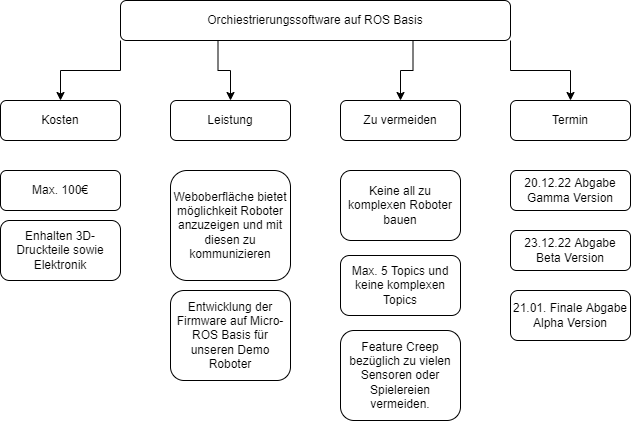
\includegraphics[width=1\textwidth]{imgs/Zielsetzung.png}
        \caption{Anforderung Diagram}
        \label{fig:dia_anforderung}%
    \end{figure}

    Kosten:
    \begin{itemize}
    \item Endkosten belaufen sich auf weniger als 100€.
    \item In diesen Kosten soll der Microcontroller inkl. 3D-Druck und gesamter Elektronik inkludiert sein.
    \end{itemize}

    Leistung:
    \begin{itemize}
    \item Weboberfläche ist lauffähig.
    \item Roboter kann mit ROS-Messages gesteuert werden.
    \item In Eigenleistung kleine fahrbare Roboterplatform auf ESP32-basis kreieren.
    \end{itemize}
        
    Zu vermeiden:
    \begin{itemize}
    \item Keinen zu komplexen Roboter designen. (Vollständig autonom fahrender Roboter)
    \item Feature creep mit all zu vielen Sensoren gilt es zu vermeiden.
    \item Roboter Antrieb mit zu viel Technik ausstatten.
    \item Vorerst sollte nur ein Testroboter entwicklet werden.
    \item Webinterface nicht zu stark mit ROS Datentypen befüllen.
    \end {itemize}

    Termine:
    \begin{itemize}
    \item 20.11. Abgabe Gamma Version.
    \item 23.12. Abgabe Beta Version.
    \item 30.12. Feedback zu Beta Versionen.
    \item 21.01. Finale Abgabe.
    \end{itemize}
    
\end{flushleft}